\documentclass{article}\usepackage{knitr}
\makeatletter
\renewcommand{\@biblabel}[1]{\quad#1.}
\makeatother
\date{}
\bibliographystyle{plain}
\usepackage{threeparttable}
\usepackage{multirow}
\usepackage{booktabs}
\IfFileExists{upquote.sty}{\usepackage{upquote}}{}

\begin{document}

\begin{flushleft}
{\Large
\textbf{My Title}
}
\end{flushleft}




\section{Introduction}
% do not write in this section...let collaborators write in introduction.docx




% pull in introduction.tex
% section is introduction
\subsection{sub heading}

This is my introduction.\cite{green:2014}


\section{Methods}



% section is methods
\subsection{another sub heading}

I used some simple methods.


\section{Results}


% this file runs from manuscript-master







The overall mean score was 5.8. Group means are listed in Table \ref{tbl}. Figure \ref{fig} shows a histogram.

\begin{table}[H]
\centering
  \begin{threeparttable}
  \caption{My table}
  \label{tbl}
  \begin{tabular}{lrrrr}
  \toprule
   & \multicolumn{2}{c}{Treatment (n=16)} & \multicolumn{2}{c}{Control (n=14)} \\
  \cmidrule(lr){2-3} \cmidrule(lr){4-5}
  Variable & Mean & SD & Mean & SD \\
  \midrule
  % latex table generated in R 3.0.2 by xtable 1.7-1 package
% Tue Jan 28 08:46:34 2014
 Coolness & 7.8 & 0.9 & 3.4 & 0.9 \\ 
  Smarts & 29.8 & 5.0 & 25.8 & 2.9 \\ 
  
  \bottomrule
  \end{tabular}
  \begin{tablenotes}
  \small
  \item My notes
  \end{tablenotes}
  \end{threeparttable}
\end{table}




\begin{figure}[H]
  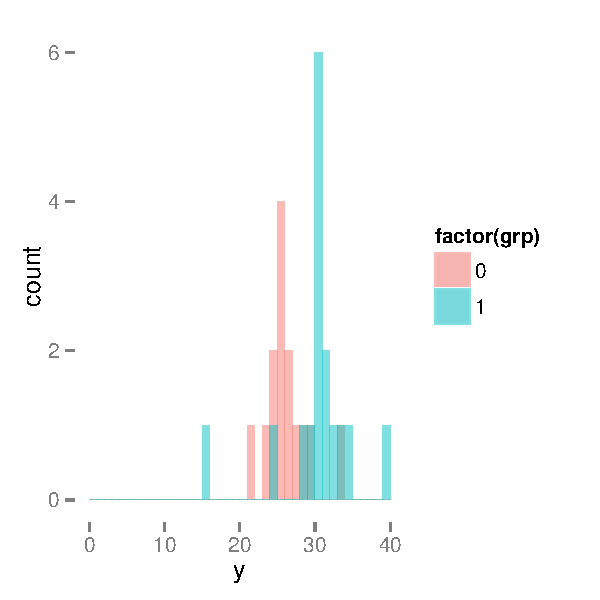
\includegraphics{output/plot.pdf}
  \caption{My figure}
  \label{fig}
\end{figure}


\section{Discussion}



% section is discussion
In conclusion, I think this works.

\subsection{limitations}

textutil is only for OSX


\bibliography{myrefs.bib}
\end{document}
